\documentclass{llncs}

% For FIGURES: (1) include figures and (2) float position of figures
\usepackage{graphicx}
\usepackage{subfigure,dblfloatfix} %to fix the problem of [h!] [t!] [!b]


\begin{document}

\title{\huge DDoS Filtering Tool\\ \small A Design Paper}

\author{Jos\'e Jair Santanna \and Julik Keijer}
\institute{University of Twente, the Netherlands\\
\email{j.j.santanna@utwente.nl \& keijerjs@gmail.com},\\ 
\texttt{http://ddosdb.org/ddosfiltering}}
\maketitle             

%\begin{abstract}
%\end{abstract}

\section{Introduction}

\section{Collaborators Requirement}

\noindent
\textsc{Main requirement:} 
\begin{itemize}
	\item Facilitate the removing of any private information that can be potentially used for identifying either the collaborators or their clients;
	\item Generate a summary of the attack and the IP addresses that are involved in the attack;
	\item Generate a new network file with only the attack records.
\end{itemize}

\noindent
\textsc{Additional requirements:}
\begin{itemize}
	\item Process the traffic at the collaborators' infrastructure to avoid leak of information;
	\item Facilitated the deployment of the filtering tool; 
	\item Speedup the loading process of visualizations;
	\item Create simple and meaningful visualizations;
	\item Have a dynamic (and manual) filtering interface;
	\item Highlight outliers.
\end{itemize}

\section{Tasks \& Modules}

The steps needed to achieve the main requirement are the following:
\begin{enumerate}
	\item Receive an uploaded network file that contains a DDoS attack (pcap[ng] or nfdump types);	
	\item Pre-filter the uploaded network file keeping only the ingress traffic;
	\item Highlight the potential attack targets, i.e., the destination IP addresses that received more network traffic);
	\item Highlight the IP protocol that generates more network traffic towards the highlighted destination IP address;
	\item Present summarized information of source IPs that sent traffic using the highlighted IP protocol;
	\item Highlight (and manually remove) the source IPs that does not follow an attack pattern (outliers);
	\item Classify the set of remaining source IPs as a type of DDoS attack;
	\item[*8.] Use the set of remaining source IPs to filter the pre-filtered traffic (output of step 2) towards identify multi-vector attacks;  
	\item[9.] Repeat steps 3, 4, 5 and 6 until the collaborator is satisfied about the remaining information;
	\item[10.] Generate a new network attack file with only the remaining information;
	\item[11.] Export the new network attack file and the summary of the attack to DDoSDB.
\end{enumerate}

\begin{figure}[!ht] 
\centering 
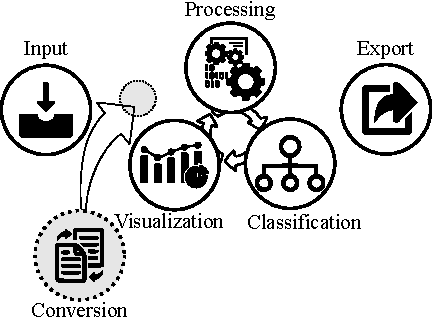
\includegraphics[]{figs/modules.pdf}
\caption{DDoS filtering tool modules.} 
\label{fig:modules} 
\end{figure}

Web-based that performs offline filtering;

\section{Preliminary results}
\end{document}
